% This file was converted to LaTeX by Writer2LaTeX ver. 1.9.9
% see http://writer2latex.sourceforge.net for more info
\documentclass[letterpaper]{report}
\usepackage{calc,amsmath,amssymb,amsfonts}
\usepackage[T1]{fontenc}
\usepackage[english]{babel}
\usepackage{xcolor}
\usepackage[top=2cm,bottom=1.27cm,left=3cm,right=2cm,includefoot]{geometry}
\usepackage[style=numeric,backend=biber]{biblatex}
\usepackage{array,supertabular,hhline,hyperref}
\hypersetup{colorlinks=true,allcolors=blue,pdftitle=SDD Template,pdfauthor=Bui Hoang Tu 20200547}
\usepackage[pdftex]{graphicx}
\setlength\tabcolsep{1mm}
\renewcommand\arraystretch{1.3}
\title{SDD Template}
\author{Bui Hoang Tu 20200547}
\date{2023-10-15}
\begin{document}
\clearpage

HANOI UNIVERSITY OF SCIENCE AND TECHNOLOGY

School of Information and Communications Technology


\bigskip

Software Requirement Specification

Version 1.1


\bigskip


\bigskip

AIMS

Subject: Phân tích và thi[1EBF?]t k[1EBF?] h[1EC7?] th[1ED1?]ng


\bigskip


\bigskip


\bigskip

Bùi Hoàng Tú 20200547 


\bigskip


\bigskip


\bigskip


\bigskip

\textit{Hanoi}


\bigskip
\endinput

\clearpage\clearpage
\chapter{Table of contents}

\bigskip

\setcounter{tocdepth}{3}
\tableofcontents

\bigskip

\chapter{Introduction}
\section{Objective}
This document presents the detailed description for User management subsystem, user group and their usable function at run time. This document also describes the objectives and features of the system, interfaces and constraints of the system in response to external action.

This document is for stakeholders and related software developers.

\section{Scope}

\bigskip

\section{Glossary}
\section{References}
\chapter{Overall requirements}
\section{Actors}
\begin{itemize}
\item Admin: Staffs who manage the store
\item User: Clients who use buy the products
\item VNPay: Paying port 
\end{itemize}

\bigskip


\bigskip

\clearpage\section{General use case diagram}
 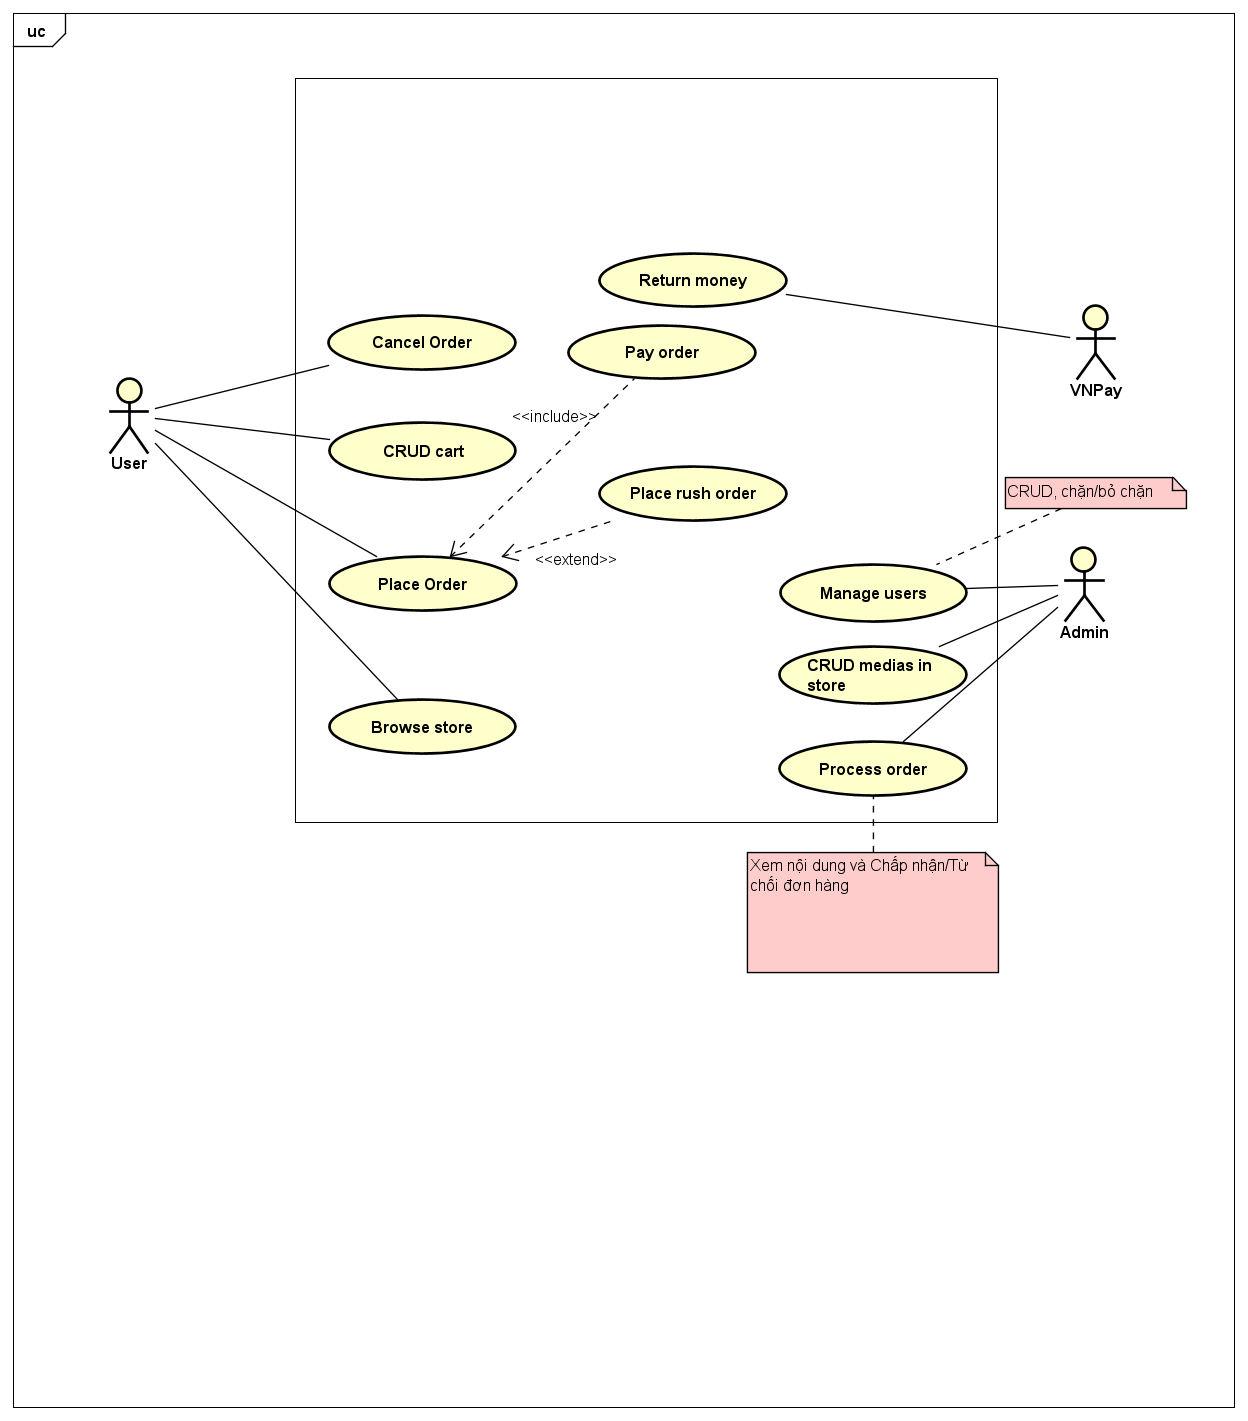
\includegraphics[width=15.24cm,height=17.353cm]{UseCaseSpecification-img/UseCaseSpecification-img001.png} 

\section{Business processes \ \ \ \ \ \ \ \ }
 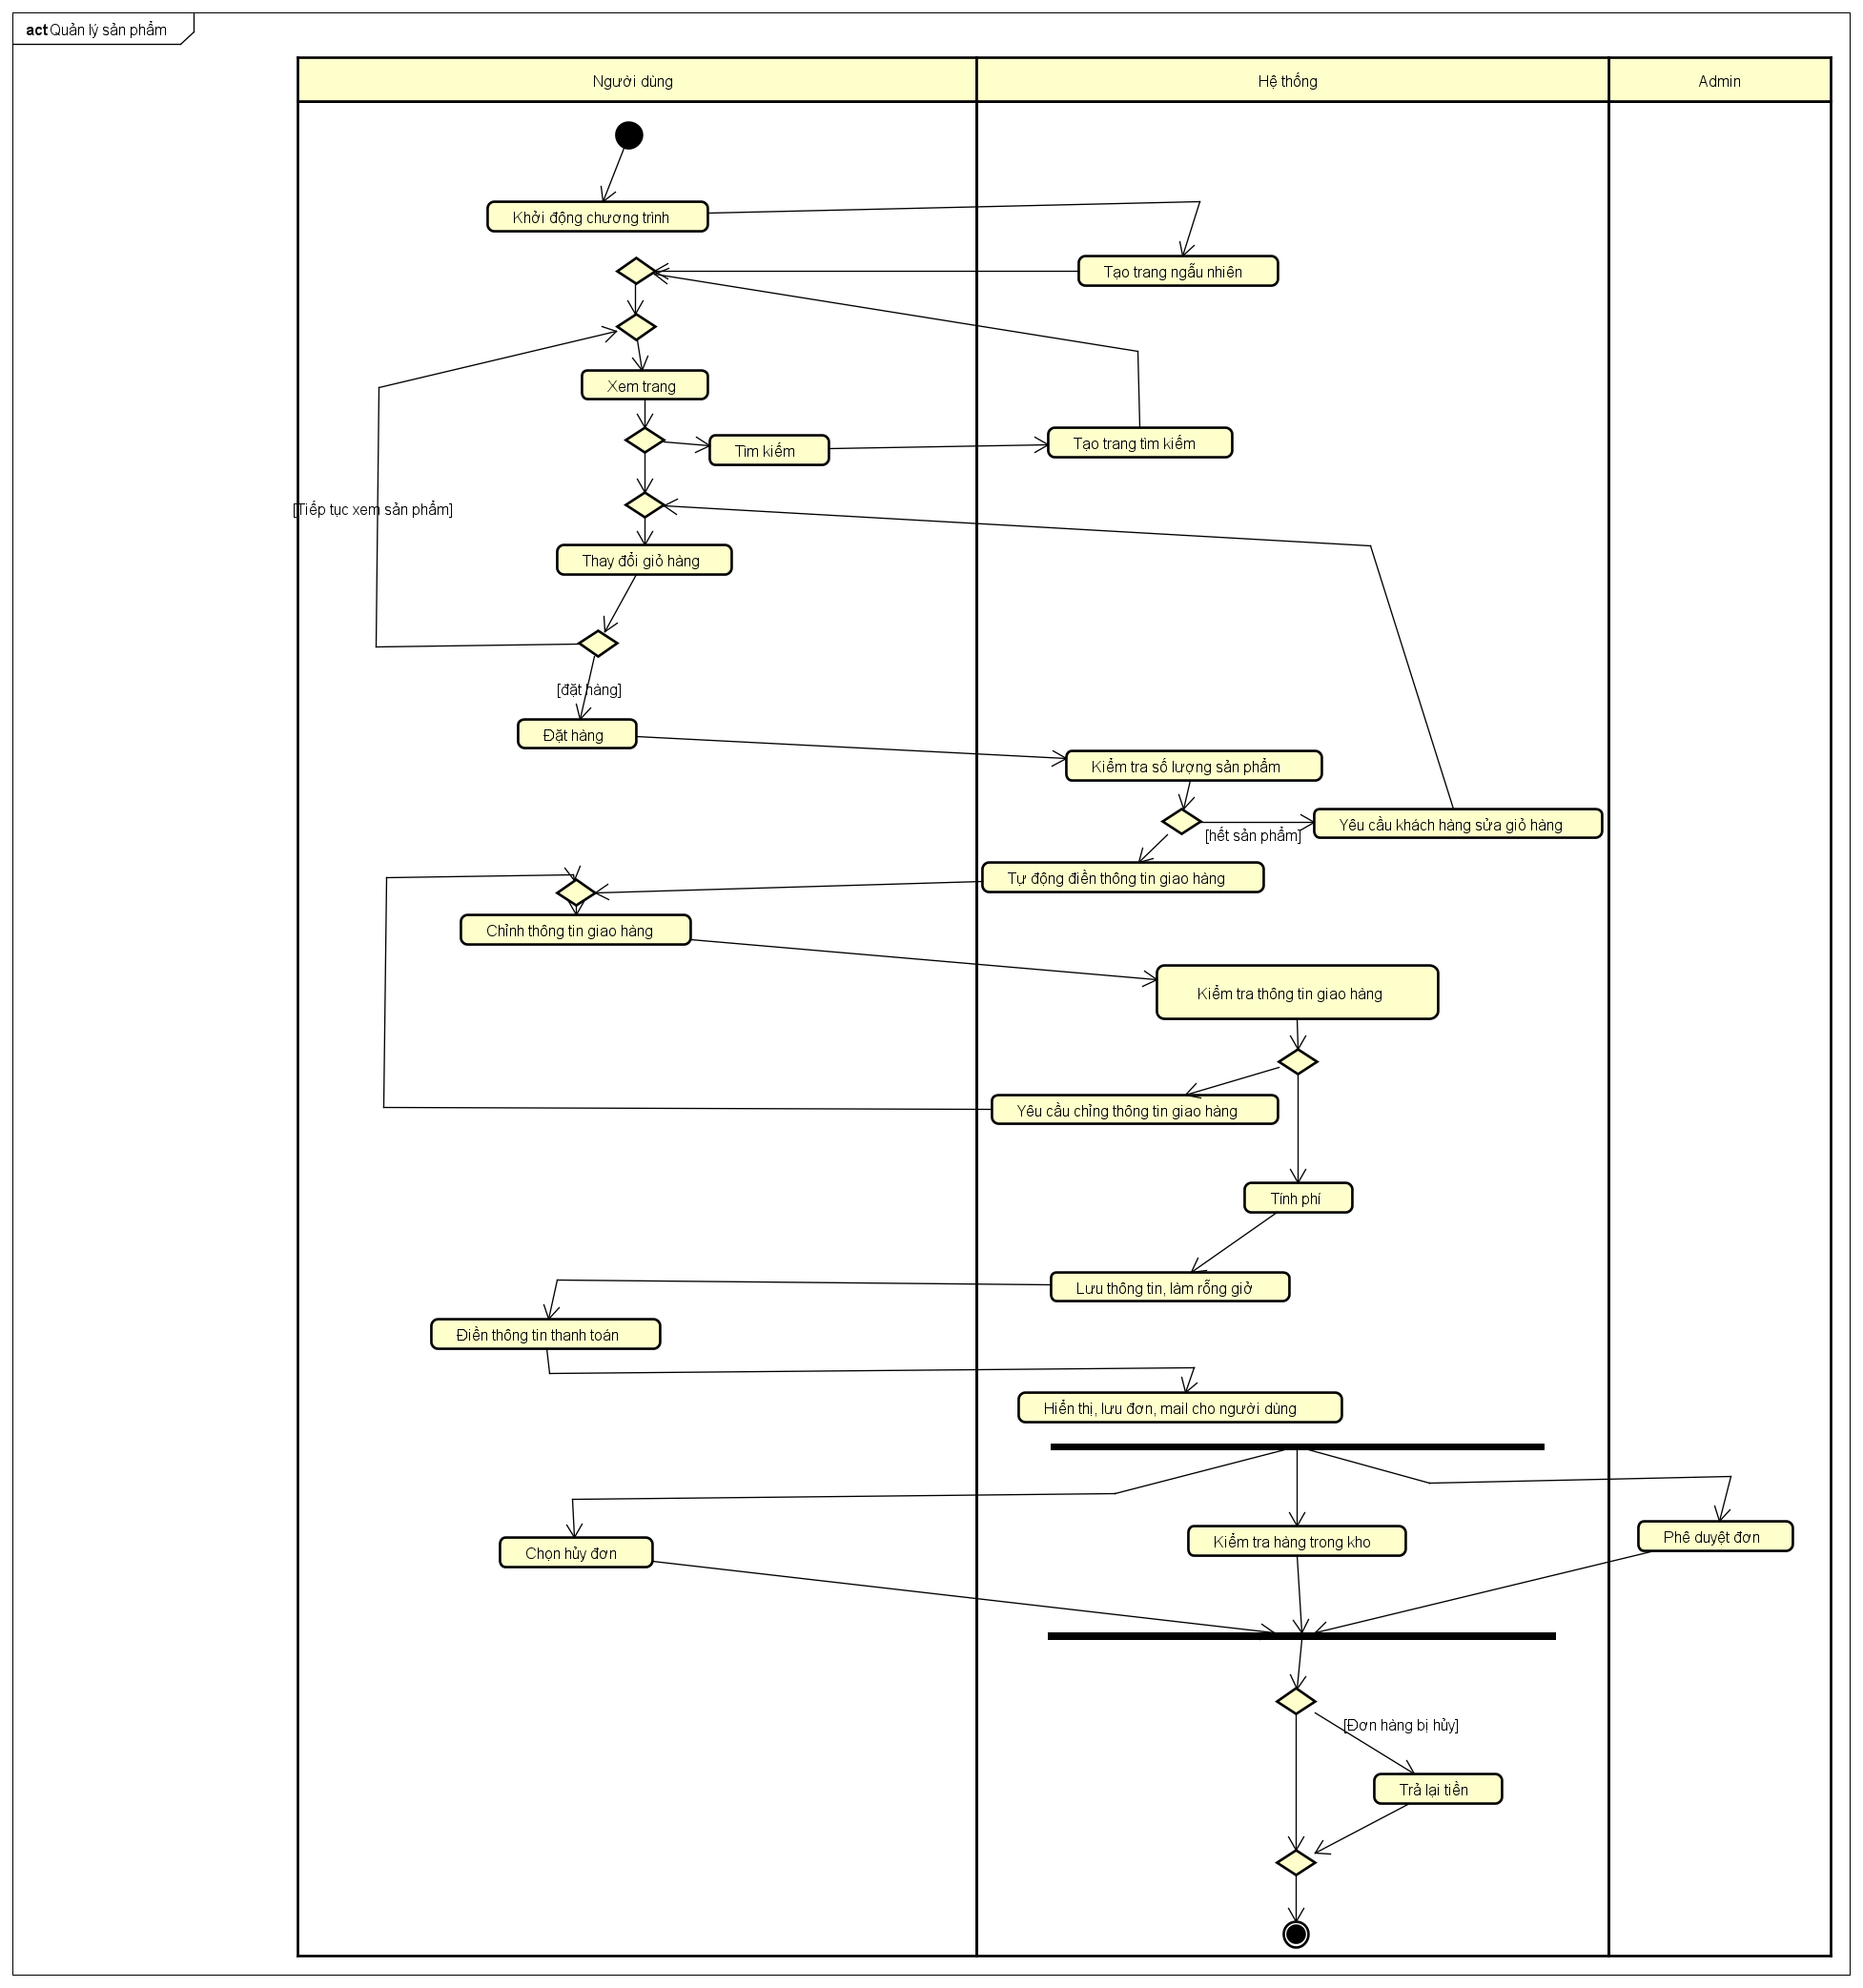
\includegraphics[width=15.24cm,height=16.261cm]{UseCaseSpecification-img/UseCaseSpecification-img002.png} 

\chapter{Detail requirements}
Details of the use cases given in following sections are specified below.


\bigskip

\section[Specification of Use case UC001 {}- “Place Order”]{Specification of Use case UC001 - “Place Order”}
\begin{enumerate}
\item \textbf{Use case code}
\end{enumerate}
UC001

\begin{enumerate}
\item \textbf{Brief Description}
\end{enumerate}
\ UC “Place Order” describes he interaction between customers and AIMS software when the customer wishes to place order

\begin{enumerate}
\item \textbf{Actors}
\end{enumerate}
\begin{itemize}
\item User
\end{itemize}
\begin{enumerate}
\item \textbf{Preconditions}
\end{enumerate}
No

\begin{enumerate}
\item \textbf{Basic Flow of Events}
\end{enumerate}
\begin{enumerate}
\item The customer requests to place order in the cart 
\item The AIMS software checks the availability of products in the cart 
\item The AIMS software displays the form of delivery information 
\item The customer enters and submits delivery information 
\item The AIMS software calculates shipping fees 
\item The AIMS software displays the invoice 
\item The customer confirms to place order 
\item The AIMS software calls UC “Pay order” 
\item \ The AIMS software creates a new order 
\item The AIMS software makes the cart empty 
\item The AIMS software sends email about the order notification and information 
\item The AIMS software displays successful order notification and the order information
\end{enumerate}
\begin{enumerate}
\item \textbf{Alternative flows}
\end{enumerate}
{\bfseries
Table Alternative flows of events for UC Place order}

\begin{flushleft}
\tablefirsthead{}
\tablehead{}
\tabletail{}
\tablelasttail{}
\begin{supertabular}{|m{0.85999995cm}|m{1.513cm}|m{3.148cm}|m{7.1200004cm}|m{1.98cm}|}
\hline
\foreignlanguage{english}{\textbf{No}} &
\foreignlanguage{english}{\textbf{Locatio}}\foreignlanguage{english}{\textbf{n}} &
\foreignlanguage{english}{\textbf{Condition}} &
\foreignlanguage{english}{\textbf{Action}} &
\foreignlanguage{english}{\textbf{Resume }}\foreignlanguage{english}{\textbf{location}}\\\hline
\begin{enumerate}
\item ~
\end{enumerate}
 &
\foreignlanguage{english}{Step 2} &
\foreignlanguage{english}{If product is not available} &
\begin{itemize}
\item \foreignlanguage{english}{Notifies users then navigate them to “View Cart”}\end{itemize}
 &
\foreignlanguage{english}{End}\\\hline
\begin{enumerate}
\item ~
\end{enumerate}
 &
Step \foreignlanguage{english}{4} &
If the delivery info is invalid &
\begin{itemize}
\item notifies that the delivery info is invalid (blank or wrong format\end{itemize}
 &
\foreignlanguage{english}{Step 3}\\\hline
\begin{enumerate}
\item ~
\end{enumerate}
 &
Step \foreignlanguage{english}{4} &
If the user chooses to place a rush order &
\begin{itemize}
\item \foreignlanguage{english}{Navigate user to UC003}\end{itemize}
 &
Step 5\\\hline
\begin{enumerate}
\item ~
\end{enumerate}
 &
Step \foreignlanguage{english}{8} &
If the order payment is not successful &
\begin{itemize}
\item notifies that the payment is not successful\end{itemize}
 &
\foreignlanguage{english}{Step 7}\\\hline
\end{supertabular}
\end{flushleft}

\bigskip


\bigskip

\begin{enumerate}
\item \textbf{Input data}
\end{enumerate}
{\bfseries
Table Input data of delivery information}

\begin{flushleft}
\tablefirsthead{}
\tablehead{}
\tabletail{}
\tablelasttail{}
\begin{supertabular}{|m{0.744cm}|m{2.181cm}|m{2.34cm}|m{2.181cm}|m{3.291cm}|m{4.086cm}|}
\hline
\foreignlanguage{english}{\textbf{No}} &
\foreignlanguage{english}{\textbf{Data fields}} &
\foreignlanguage{english}{\textbf{Description}} &
\foreignlanguage{english}{\textbf{Mandatory}} &
\foreignlanguage{english}{\textbf{Valid condition}} &
\foreignlanguage{english}{\textbf{Example}}\\\hline
\begin{enumerate}
\item ~
\end{enumerate}
 &
Receiver Name &
~
 &
Yes &
~
 &
\foreignlanguage{english}{Bui Hoang Tu}\\\hline
\begin{enumerate}
\item ~
\end{enumerate}
 &
\foreignlanguage{english}{P}hone Number &
~
 &
Yes &
\foreignlanguage{english}{10 digits} &
\foreignlanguage{english}{0987 654 321}\\\hline
\begin{enumerate}
\item ~
\end{enumerate}
 &
Province &
\foreignlanguage{english}{Choose from list} &
Yes &
~
 &
\foreignlanguage{english}{Hanoi}\\\hline
\begin{enumerate}
\item ~
\end{enumerate}
 &
Address &
~
 &
Yes &
~
 &
\foreignlanguage{english}{12/18 Dai Co Viet street, Hai Ba Trung district}\\\hline
\begin{enumerate}
\item ~
\end{enumerate}
 &
Shipping instructions &
~
 &
\foreignlanguage{english}{No} &
~
 &
\foreignlanguage{english}{Drive in for about 100m}\\\hline
\end{supertabular}
\end{flushleft}

\bigskip

\begin{enumerate}
\item \textbf{Output data}
\end{enumerate}
{\bfseries
Table B-Output data of \ displaying invoice}

The first 4 rows are repeated for each product

\begin{flushleft}
\tablefirsthead{}
\tablehead{}
\tabletail{}
\tablelasttail{}
\begin{supertabular}{|m{0.902cm}|m{2.181cm}|m{3.769cm}|m{4.5610003cm}|m{3.612cm}|}
\hline
\foreignlanguage{english}{\textbf{No}} &
\foreignlanguage{english}{\textbf{Data fields}} &
\foreignlanguage{english}{\textbf{Description}} &
\foreignlanguage{english}{\textbf{Display format}} &
\foreignlanguage{english}{\textbf{Example}}\\\hline
\begin{enumerate}
\item ~
\end{enumerate}
 &
Title &
Title of a media product &
~
 &
\foreignlanguage{english}{DVD Phim A}\\\hline
\begin{enumerate}
\item ~
\end{enumerate}
 &
Price &
Price of the corresponding media product &
\begin{itemize}
\item \foreignlanguage{english}{Dot }for thousands separator\item Right alignment\end{itemize}
 &
\foreignlanguage{english}{10.000}\\\hline
\begin{enumerate}
\item ~
\end{enumerate}
 &
Quantity &
Quantity of the corresponding media &
Right alignmen\foreignlanguage{english}{t} &
\foreignlanguage{english}{3}\\\hline
\begin{enumerate}
\item ~
\end{enumerate}
 &
Amount &
Total money of the corresponding medi\foreignlanguage{english}{a} &
•\ \ Dot for thousands separator

•\ \ Right alignment &
\foreignlanguage{english}{100.000}\\\hline
\begin{enumerate}
\item ~
\end{enumerate}
 &
Subtotal Before VAT &
Total price of products in the cart before VAT &
•\ \ Dot for thousands separator

•\ \ Right alignment &
\foreignlanguage{english}{1.000.000}\\\hline
\begin{enumerate}
\item ~
\end{enumerate}
 &
Subtotal &
Total price of products in the cart with VAT &
~
 &
\foreignlanguage{english}{1.100.00}\\\hline
\begin{enumerate}
\item ~
\end{enumerate}
 &
Shipping fees &
~
 &
~
 &
\foreignlanguage{english}{37.000}\\\hline
\begin{enumerate}
\item ~
\end{enumerate}
 &
Total &
Sum of subtotal and shipping fees &
~
 &
\foreignlanguage{english}{1.137.00}\\\hline
\begin{enumerate}
\item ~
\end{enumerate}
 &
Currency &
~
 &
~
 &
\foreignlanguage{english}{VND}\\\hline
\begin{enumerate}
\item ~
\end{enumerate}
 &
Name &
~
 &
~
 &
\foreignlanguage{english}{Bui Hoang Tu}\\\hline
\begin{enumerate}
\item ~
\end{enumerate}
 &
Phone number &
~
 &
~
 &
\foreignlanguage{english}{0987654321}\\\hline
\begin{enumerate}
\item ~
\end{enumerate}
 &
Province &
~
 &
~
 &
\foreignlanguage{english}{Hanoi}\\\hline
\begin{enumerate}
\item ~
\end{enumerate}
 &
Address &
~
 &
~
 &
\foreignlanguage{english}{12/18 Dai Co Viet street, Hai Ba Trung district}\\\hline
\begin{enumerate}
\item ~
\end{enumerate}
 &
\foreignlanguage{english}{S}hipping instructions &
~
 &
~
 &
\foreignlanguage{english}{Drive in for about 100m}\\\hline
\end{supertabular}
\end{flushleft}

\bigskip


\bigskip

\section[Specification of Use case UC002 {}- “Pay order”]{Specification of Use case UC002 - “Pay order”}
\begin{enumerate}
\item \textbf{Use case code}
\end{enumerate}
UC002

\begin{enumerate}
\item \textbf{Brief Description}
\end{enumerate}
This use case describes the interaction between users and the AIMS software and VNPay when the customer wishes to pay his/her order.

\begin{enumerate}
\item \textbf{Actors}
\end{enumerate}
\begin{enumerate}
\item User
\item VNPay
\end{enumerate}
\begin{enumerate}
\item \textbf{Preconditions}
\end{enumerate}
The AIMS software has calculated the total amount of money which the customer has to pay.

\begin{enumerate}
\item \textbf{Basic Flow of Events}
\end{enumerate}
\begin{enumerate}
\item The AIMS software displays the payment screen
\item The customer enters credit card info and confirms to pay order
\item The AIMS software asks the Interbank to process the payment transaction
\item The Interbank processes the payment transaction
\item The AIMS software saves the payment transaction
\item The AIMS software displays transaction information
\item The AIMS software sends e-mail to the customer
\end{enumerate}
\begin{enumerate}
\item \textbf{Alternative flows}
\end{enumerate}
{\bfseries
Table N-Alternative flows of events for UC Place order}

\begin{flushleft}
\tablefirsthead{}
\tablehead{}
\tabletail{}
\tablelasttail{}
\begin{supertabular}{|m{0.87200004cm}|m{1.918cm}|m{3.3cm}|m{5.803cm}|m{2.728cm}|}
\hline
\foreignlanguage{english}{\textbf{No}} &
\foreignlanguage{english}{\textbf{Location}} &
\foreignlanguage{english}{\textbf{Condition}} &
\foreignlanguage{english}{\textbf{Action}} &
\foreignlanguage{english}{\textbf{Resume location}}\\\hline
\begin{enumerate}
\item ~
\end{enumerate}
 &
\foreignlanguage{english}{At Step 3} &
\foreignlanguage{english}{If the card info is in invalid} &
\begin{itemize}
\item \foreignlanguage{english}{The AIMS software notifies that the card info is invalid}\end{itemize}
 &
\foreignlanguage{english}{At Step 1}\\\hline
\begin{enumerate}
\item ~
\end{enumerate}
 &
At Step \foreignlanguage{english}{4} &
If the card info is wrong &
\begin{itemize}
\item \foreignlanguage{english}{The AIMS software notifies that the card info }\foreignlanguage{english}{is wrong}\end{itemize}
 &
\foreignlanguage{english}{At Step 1}\\\hline
\begin{enumerate}
\item ~
\end{enumerate}
 &
At Step \foreignlanguage{english}{4} &
If the balance is not enough &
\begin{itemize}
\item The AIMS software notifies that the balance is not enough\end{itemize}
 &
\foreignlanguage{english}{At Step 1}\\\hline
\end{supertabular}
\end{flushleft}

\bigskip


\bigskip

\begin{enumerate}
\item \textbf{Input data}
\end{enumerate}
{\bfseries
Table Input data of credit card information}

\begin{flushleft}
\tablefirsthead{}
\tablehead{}
\tabletail{}
\tablelasttail{}
\begin{supertabular}{|m{0.744cm}|m{2.181cm}|m{2.165cm}|m{2.052cm}|m{3.5939999cm}|m{4.086cm}|}
\hline
\foreignlanguage{english}{\textbf{No}} &
\foreignlanguage{english}{\textbf{Data fields}} &
\foreignlanguage{english}{\textbf{Description}} &
\foreignlanguage{english}{\textbf{Mandatory}} &
\foreignlanguage{english}{\textbf{Valid condition}} &
\foreignlanguage{english}{\textbf{Example}}\\\hline
\begin{enumerate}
\item ~
\end{enumerate}
 &
Card holder name &
~
 &
Yes &
Maximum of 50 characters\foreignlanguage{english}{, all in uppercase} &
\foreignlanguage{english}{BUI HOANG TU}\\\hline
\foreignlanguage{english}{2.} &
Card number &
~
 &
Yes &
16 digits &
\foreignlanguage{english}{0123 4567 8912 3456}\\\hline
\foreignlanguage{english}{3.} &
Expiration date &
~
 &
Yes &
Consist of month and last 2 digits of year onl\foreignlanguage{english}{y} &
01/23\\\hline
\foreignlanguage{english}{4.} &
Security code &
~
 &
Yes &
3 digits &
\foreignlanguage{english}{221}\\\hline
\end{supertabular}
\end{flushleft}

\bigskip


\bigskip

\begin{enumerate}
\item \clearpage
\textbf{Output data}
\end{enumerate}
{\bfseries
Table B-Output data of …}

\begin{flushleft}
\tablefirsthead{}
\tablehead{}
\tabletail{}
\tablelasttail{}
\begin{supertabular}{|m{0.742cm}|m{2.799cm}|m{2.0509999cm}|m{5.822cm}|m{3.612cm}|}
\hline
\foreignlanguage{english}{\textbf{No}} &
\foreignlanguage{english}{\textbf{Data fields}} &
\foreignlanguage{english}{\textbf{Description}} &
\foreignlanguage{english}{\textbf{Display format}} &
\foreignlanguage{english}{\textbf{Example}}\\\hline
\begin{enumerate}
\item ~
\end{enumerate}
 &
Transaction ID &
~
 &
~
 &
~
\\\hline
\begin{enumerate}
\item ~
\end{enumerate}
 &
Card holder name &
~
 &
~
 &
\foreignlanguage{english}{BUI HOANG TU}\\\hline
\begin{enumerate}
\item ~
\end{enumerate}
 &
Amount &
\foreignlanguage{english}{Amount of money has been subtracted from your account} &
\begin{itemize}
\item \foreignlanguage{english}{Right alignment}\item \foreignlanguage{english}{With Vietnamese currency (VND)}\item \foreignlanguage{english}{Vietnam locale}\end{itemize}
 &
\foreignlanguage{english}{12.000VND}\\\hline
\begin{enumerate}
\item ~
\end{enumerate}
 &
\foreignlanguage{english}{T}ransaction Content &
~
 &
~
 &
~
\\\hline
\begin{enumerate}
\item ~
\end{enumerate}
 &
\foreignlanguage{english}{Balance} &
\foreignlanguage{english}{New balance after this transaction} &
•\ \ Right alignment

•\ \ With Vietnamese currency (VND)

•\ \ Vietnam locale &
\foreignlanguage{english}{2.300.123VND}\\\hline
\begin{enumerate}
\item ~
\end{enumerate}
 &
Transaction Date &
~
 &
\foreignlanguage{english}{dd/mm/yyyy} &
\foreignlanguage{english}{12/08/2002}\\\hline
\end{supertabular}
\end{flushleft}

\bigskip


\bigskip


\bigskip

\section[Specification of Use case UC003 {}- “Place rush order”]{Specification of Use case UC003 - “Place rush order”}
\begin{enumerate}
\item \textbf{Use case code}
\end{enumerate}
UC003

\begin{enumerate}
\item \textbf{Brief Description}
\end{enumerate}
This use case describes the interaction between users and the AIMS software and VNPay when the customer wishes to have fast delivery.

\begin{enumerate}
\item \textbf{Actors}
\end{enumerate}
\begin{enumerate}
\item User
\item VNPay
\end{enumerate}
\begin{enumerate}
\item \textbf{Preconditions}
\end{enumerate}
User choose to have fast delivery from UC001

\begin{enumerate}
\item \textbf{Basic Flow of Events}
\end{enumerate}
\begin{enumerate}
\item Users put in their address
\item The AIMS software checks the availability of service in address and items
\item AIMS asks for rush order information
\item User fills in rush information
\item Return to UC001
\end{enumerate}
\begin{enumerate}
\item \textbf{Alternative flows}
\end{enumerate}
{\bfseries
Table Alternative flows of events for UC Place order}

\begin{flushleft}
\tablefirsthead{}
\tablehead{}
\tabletail{}
\tablelasttail{}
\begin{supertabular}{|m{0.85999995cm}|m{1.513cm}|m{3.148cm}|m{7.1200004cm}|m{1.98cm}|}
\hline
\foreignlanguage{english}{\textbf{No}} &
\foreignlanguage{english}{\textbf{Location}} &
\foreignlanguage{english}{\textbf{Condition}} &
\foreignlanguage{english}{\textbf{Action}} &
\foreignlanguage{english}{\textbf{Resume location}}\\\hline
\begin{enumerate}
\item ~
\end{enumerate}
 &
\foreignlanguage{english}{Step 2} &
\foreignlanguage{english}{If address is not supported or no item support rush order} &
\begin{itemize}
\item \foreignlanguage{english}{Notifies} the error \foreignlanguage{english}{in address or no supported item}\end{itemize}
 &
\foreignlanguage{english}{Step 1}\\\hline
\end{supertabular}
\end{flushleft}

\bigskip


\bigskip

\begin{enumerate}
\item \textbf{Input data}
\end{enumerate}
{\bfseries
Table Input data of delivery information}

\begin{flushleft}
\tablefirsthead{}
\tablehead{}
\tabletail{}
\tablelasttail{}
\begin{supertabular}{|m{0.744cm}|m{2.181cm}|m{2.34cm}|m{2.181cm}|m{3.291cm}|m{4.086cm}|}
\hline
\foreignlanguage{english}{\textbf{No}} &
\foreignlanguage{english}{\textbf{Data fields}} &
\foreignlanguage{english}{\textbf{Description}} &
\foreignlanguage{english}{\textbf{Mandatory}} &
\foreignlanguage{english}{\textbf{Valid condition}} &
\foreignlanguage{english}{\textbf{Example}}\\\hline
\begin{enumerate}
\item ~
\end{enumerate}
 &
\foreignlanguage{english}{Extra }Address &
~
 &
Yes &
~
 &
\foreignlanguage{english}{12/18 Dai Co Viet street, Hai Ba Trung district}\\\hline
\begin{enumerate}
\item ~
\end{enumerate}
 &
Shipping instructions &
~
 &
\foreignlanguage{english}{No} &
~
 &
\foreignlanguage{english}{Drive in for about 100m}\\\hline
\begin{enumerate}
\item ~
\end{enumerate}
 &
\foreignlanguage{english}{Receive time} &
~
 &
\foreignlanguage{english}{Yes} &
\foreignlanguage{english}{hh:mm} &
\foreignlanguage{english}{13:34}\\\hline
\end{supertabular}
\end{flushleft}

\bigskip

\begin{enumerate}
\item \textbf{Output data}
\item \textbf{Post Condition }
\end{enumerate}

\bigskip

\chapter{Supplementary specification}
\textit{{\textless}Presenting other requirements if necessary, including non-functional requirements such as performance, reliability, usability, and supportability; or other technical requirements such as database system, used technology…{\textgreater}}

\section{Functionality}
{\textless}List of the functional requirements that are general to many use cases. E.g. Among the flow of events of use case, in all the steps that interacts with the database system, if there are errors in the connection or operation processes, there need to be a corresponding error notifications so that the actor knows that the error is related to the database system rather than the user{\textgreater}

\section{Usability}
{\textless}Requirements that relate to, or affect, the usability of the software. Examples include ease-of-use requirements or training requirements that specify how readily the software can be used by its actors{\textgreater}

\section{Reliability}
{\textless}Any requirements concerning the reliability of the software. Quantitative measures such as mean time between failure or defects per thousand lines of code should be stated{\textgreater}

\section{Performance}
{\textless}The performance characteristics of the software. \ Include specific response times. \ Reference related use cases by name{\textgreater}

\section{Maintainability}
{\textless}Any requirements that will enhance the supportability or maintainability of the software being built{\textgreater}

\section{Design Constraints}
{\textless}Any design constraints on the software being built{\textgreater}
\end{document}
